\documentclass[1p]{elsarticle_modified}
%\bibliographystyle{elsarticle-num}

%\usepackage[colorlinks]{hyperref}
%\usepackage{abbrmath_seonhwa} %\Abb, \Ascr, \Acal ,\Abf, \Afrak
\usepackage{amsfonts}
\usepackage{amssymb}
\usepackage{amsmath}
\usepackage{amsthm}
\usepackage{scalefnt}
\usepackage{amsbsy}
\usepackage{kotex}
\usepackage{caption}
\usepackage{subfig}
\usepackage{color}
\usepackage{graphicx}
\usepackage{xcolor} %% white, black, red, green, blue, cyan, magenta, yellow
\usepackage{float}
\usepackage{setspace}
\usepackage{hyperref}

\usepackage{tikz}
\usetikzlibrary{arrows}

\usepackage{multirow}
\usepackage{array} % fixed length table
\usepackage{hhline}

%%%%%%%%%%%%%%%%%%%%%
\makeatletter
\renewcommand*\env@matrix[1][\arraystretch]{%
	\edef\arraystretch{#1}%
	\hskip -\arraycolsep
	\let\@ifnextchar\new@ifnextchar
	\array{*\c@MaxMatrixCols c}}
\makeatother %https://tex.stackexchange.com/questions/14071/how-can-i-increase-the-line-spacing-in-a-matrix
%%%%%%%%%%%%%%%

\usepackage[normalem]{ulem}

\newcommand{\msout}[1]{\ifmmode\text{\sout{\ensuremath{#1}}}\else\sout{#1}\fi}
%SOURCE: \msout is \stkout macro in https://tex.stackexchange.com/questions/20609/strikeout-in-math-mode

\newcommand{\cancel}[1]{
	\ifmmode
	{\color{red}\msout{#1}}
	\else
	{\color{red}\sout{#1}}
	\fi
}

\newcommand{\add}[1]{
	{\color{blue}\uwave{#1}}
}

\newcommand{\replace}[2]{
	\ifmmode
	{\color{red}\msout{#1}}{\color{blue}\uwave{#2}}
	\else
	{\color{red}\sout{#1}}{\color{blue}\uwave{#2}}
	\fi
}

\newcommand{\Sol}{\mathcal{S}} %segment
\newcommand{\D}{D} %diagram
\newcommand{\A}{\mathcal{A}} %arc


%%%%%%%%%%%%%%%%%%%%%%%%%%%%%5 test

\def\sl{\operatorname{\textup{SL}}(2,\Cbb)}
\def\psl{\operatorname{\textup{PSL}}(2,\Cbb)}
\def\quan{\mkern 1mu \triangleright \mkern 1mu}

\theoremstyle{definition}
\newtheorem{thm}{Theorem}[section]
\newtheorem{prop}[thm]{Proposition}
\newtheorem{lem}[thm]{Lemma}
\newtheorem{ques}[thm]{Question}
\newtheorem{cor}[thm]{Corollary}
\newtheorem{defn}[thm]{Definition}
\newtheorem{exam}[thm]{Example}
\newtheorem{rmk}[thm]{Remark}
\newtheorem{alg}[thm]{Algorithm}

\newcommand{\I}{\sqrt{-1}}
\begin{document}

%\begin{frontmatter}
%
%\title{Boundary parabolic representations of knots up to 8 crossings}
%
%%% Group authors per affiliation:
%\author{Yunhi Cho} 
%\address{Department of Mathematics, University of Seoul, Seoul, Korea}
%\ead{yhcho@uos.ac.kr}
%
%
%\author{Seonhwa Kim} %\fnref{s_kim}}
%\address{Center for Geometry and Physics, Institute for Basic Science, Pohang, 37673, Korea}
%\ead{ryeona17@ibs.re.kr}
%
%\author{Hyuk Kim}
%\address{Department of Mathematical Sciences, Seoul National University, Seoul 08826, Korea}
%\ead{hyukkim@snu.ac.kr}
%
%\author{Seokbeom Yoon}
%\address{Department of Mathematical Sciences, Seoul National University, Seoul, 08826,  Korea}
%\ead{sbyoon15@snu.ac.kr}
%
%\begin{abstract}
%We find all boundary parabolic representation of knots up to 8 crossings.
%
%\end{abstract}
%\begin{keyword}
%    \MSC[2010] 57M25 
%\end{keyword}
%
%\end{frontmatter}

%\linenumbers
%\tableofcontents
%
\newcommand\colored[1]{\textcolor{white}{\rule[-0.35ex]{0.8em}{1.4ex}}\kern-0.8em\color{red} #1}%
%\newcommand\colored[1]{\textcolor{white}{ #1}\kern-2.17ex	\textcolor{white}{ #1}\kern-1.81ex	\textcolor{white}{ #1}\kern-2.15ex\color{red}#1	}

{\Large $\underline{12a_{0031}~(K12a_{0031})}$}

\setlength{\tabcolsep}{10pt}
\renewcommand{\arraystretch}{1.6}
\vspace{1cm}\begin{tabular}{m{100pt}>{\centering\arraybackslash}m{274pt}}
\multirow{5}{120pt}{
	\centering
	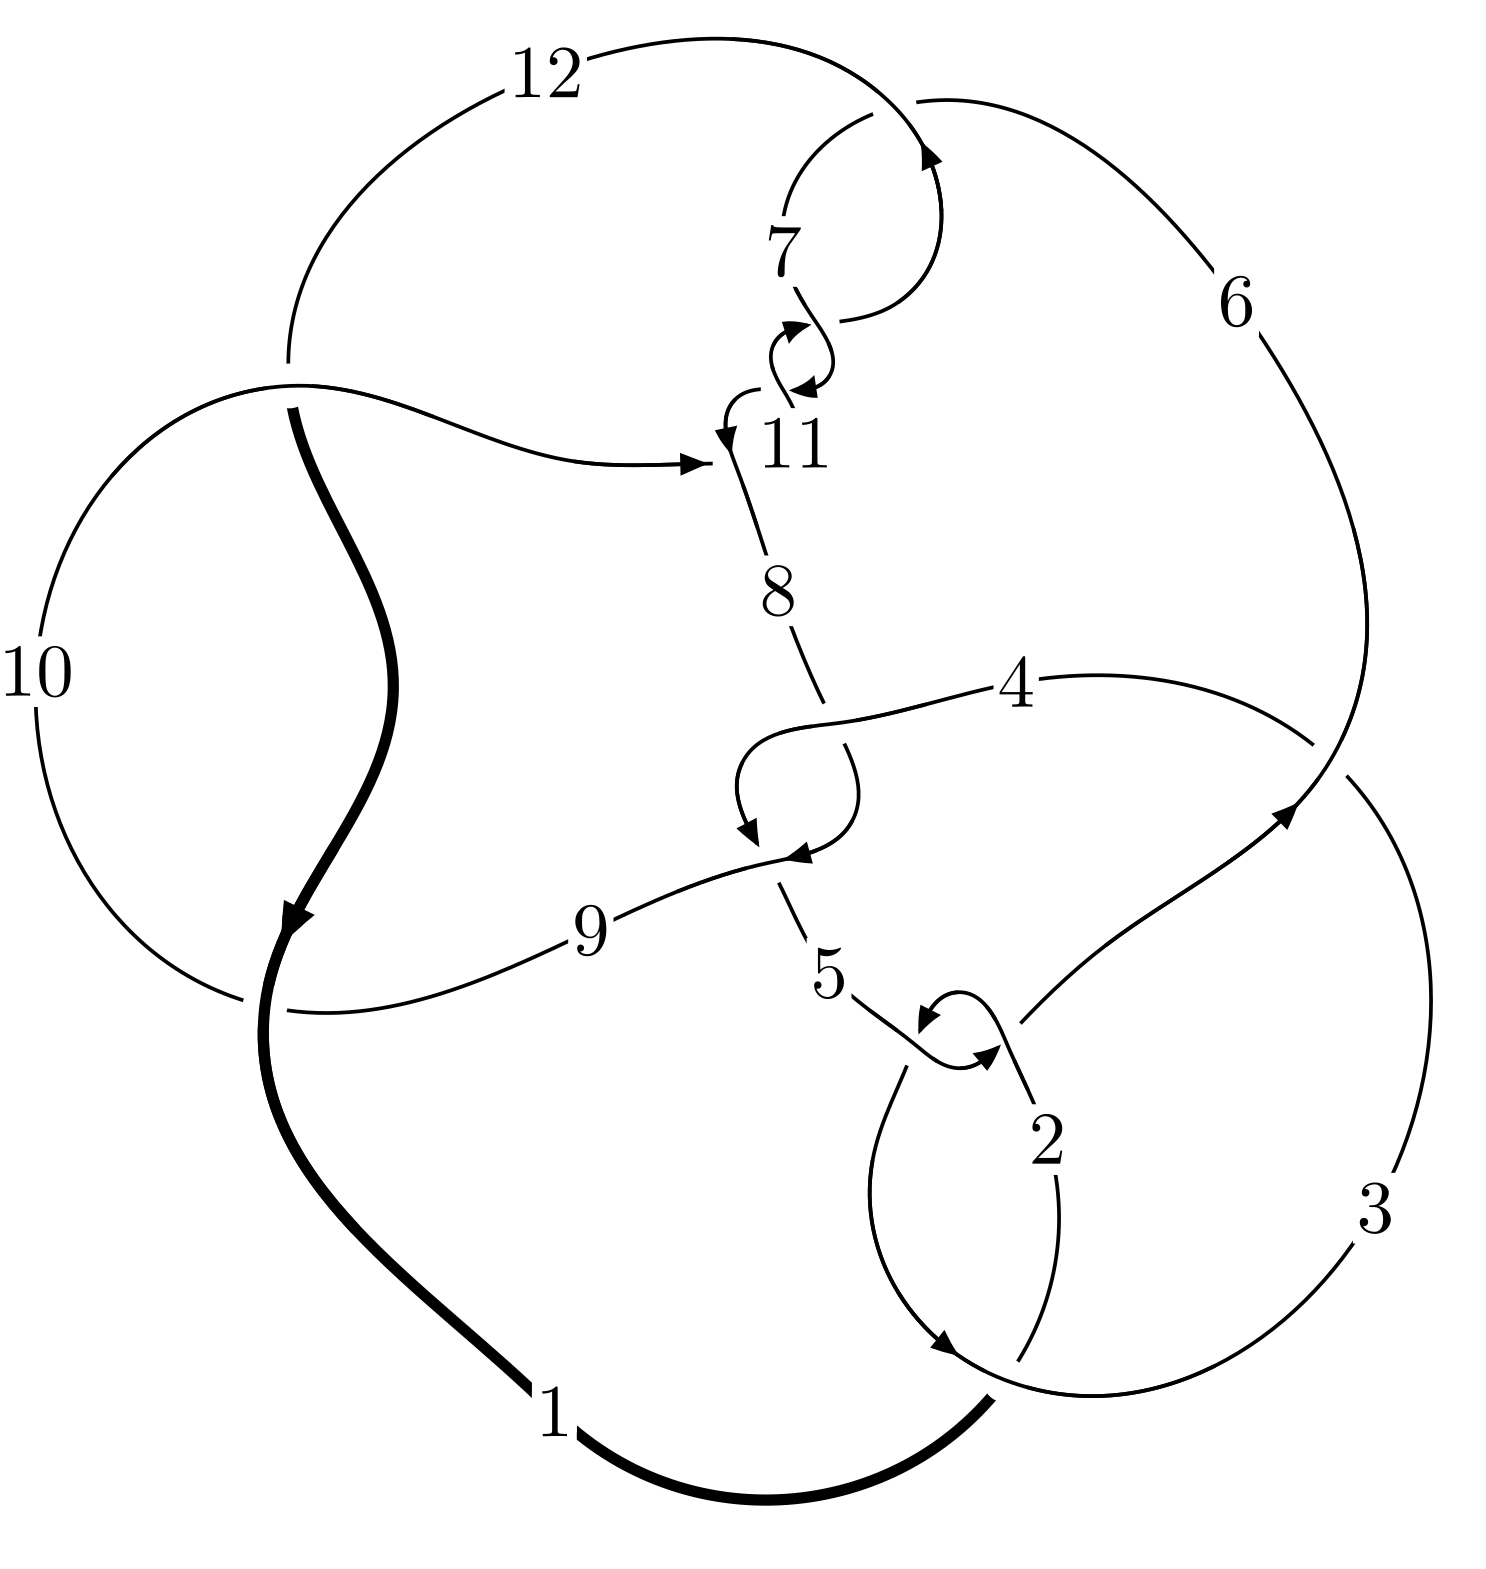
\includegraphics[width=112pt]{../../../GIT/diagram.site/Diagrams/png/832_12a_0031.png}\\
\ \ \ A knot diagram\footnotemark}&
\allowdisplaybreaks
\textbf{Linearized knot diagam} \\
\cline{2-2}
 &
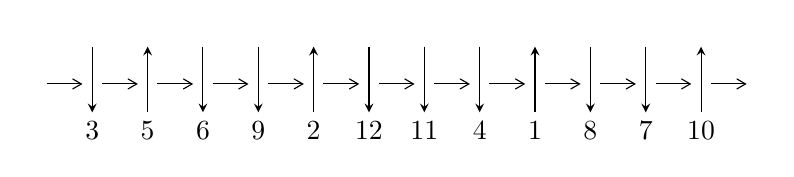
\begin{tikzpicture}[x=20pt, y=17pt]
	% nodes
	\node (C0) at (0, 0) {};
	\node (C1) at (1, 0) {};
	\node (C1U) at (1, +1) {};
	\node (C1D) at (1, -1) {3};

	\node (C2) at (2, 0) {};
	\node (C2U) at (2, +1) {};
	\node (C2D) at (2, -1) {5};

	\node (C3) at (3, 0) {};
	\node (C3U) at (3, +1) {};
	\node (C3D) at (3, -1) {6};

	\node (C4) at (4, 0) {};
	\node (C4U) at (4, +1) {};
	\node (C4D) at (4, -1) {9};

	\node (C5) at (5, 0) {};
	\node (C5U) at (5, +1) {};
	\node (C5D) at (5, -1) {2};

	\node (C6) at (6, 0) {};
	\node (C6U) at (6, +1) {};
	\node (C6D) at (6, -1) {12};

	\node (C7) at (7, 0) {};
	\node (C7U) at (7, +1) {};
	\node (C7D) at (7, -1) {11};

	\node (C8) at (8, 0) {};
	\node (C8U) at (8, +1) {};
	\node (C8D) at (8, -1) {4};

	\node (C9) at (9, 0) {};
	\node (C9U) at (9, +1) {};
	\node (C9D) at (9, -1) {1};

	\node (C10) at (10, 0) {};
	\node (C10U) at (10, +1) {};
	\node (C10D) at (10, -1) {8};

	\node (C11) at (11, 0) {};
	\node (C11U) at (11, +1) {};
	\node (C11D) at (11, -1) {7};

	\node (C12) at (12, 0) {};
	\node (C12U) at (12, +1) {};
	\node (C12D) at (12, -1) {10};
	\node (C13) at (13, 0) {};

	% arrows
	\draw[->,>={angle 60}]
	(C0) edge (C1) (C1) edge (C2) (C2) edge (C3) (C3) edge (C4) (C4) edge (C5) (C5) edge (C6) (C6) edge (C7) (C7) edge (C8) (C8) edge (C9) (C9) edge (C10) (C10) edge (C11) (C11) edge (C12) (C12) edge (C13) ;	\draw[->,>=stealth]
	(C1U) edge (C1D) (C2D) edge (C2U) (C3U) edge (C3D) (C4U) edge (C4D) (C5D) edge (C5U) (C6U) edge (C6D) (C7U) edge (C7D) (C8U) edge (C8D) (C9D) edge (C9U) (C10U) edge (C10D) (C11U) edge (C11D) (C12D) edge (C12U) ;
	\end{tikzpicture} \\
\hhline{~~} \\& 
\textbf{Solving Sequence} \\ \cline{2-2} 
 &
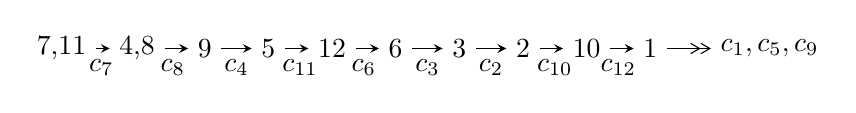
\begin{tikzpicture}[x=23pt, y=7pt]
	% node
	\node (A0) at (-1/8, 0) {7,11};
	\node (A1) at (17/16, 0) {4,8};
	\node (A2) at (17/8, 0) {9};
	\node (A3) at (25/8, 0) {5};
	\node (A4) at (33/8, 0) {12};
	\node (A5) at (41/8, 0) {6};
	\node (A6) at (49/8, 0) {3};
	\node (A7) at (57/8, 0) {2};
	\node (A8) at (65/8, 0) {10};
	\node (A9) at (73/8, 0) {1};
	\node (C1) at (1/2, -1) {$c_{7}$};
	\node (C2) at (13/8, -1) {$c_{8}$};
	\node (C3) at (21/8, -1) {$c_{4}$};
	\node (C4) at (29/8, -1) {$c_{11}$};
	\node (C5) at (37/8, -1) {$c_{6}$};
	\node (C6) at (45/8, -1) {$c_{3}$};
	\node (C7) at (53/8, -1) {$c_{2}$};
	\node (C8) at (61/8, -1) {$c_{10}$};
	\node (C9) at (69/8, -1) {$c_{12}$};
	\node (A10) at (11, 0) {$c_{1},c_{5},c_{9}$};

	% edge
	\draw[->,>=stealth]	
	(A0) edge (A1) (A1) edge (A2) (A2) edge (A3) (A3) edge (A4) (A4) edge (A5) (A5) edge (A6) (A6) edge (A7) (A7) edge (A8) (A8) edge (A9) ;
	\draw[->>,>={angle 60}]	
	(A9) edge (A10);
\end{tikzpicture} \\ 

\end{tabular} \\

\footnotetext{
The image of knot diagram is generated by the software ``\textbf{Draw programme}" developed by Andrew Bartholomew(\url{http://www.layer8.co.uk/maths/draw/index.htm\#Running-draw}), where we modified some parts for our purpose(\url{https://github.com/CATsTAILs/LinksPainter}).
}\phantom \\ \newline 
\centering \textbf{Ideals for irreducible components\footnotemark of $X_{\text{par}}$} 
 
\begin{align*}
I^u_{1}&=\langle 
-2 u^{76}-8 u^{75}+\cdots+2 b-2,\;u^{76}+3 u^{75}+\cdots+2 a+4,\;u^{77}+3 u^{76}+\cdots-5 u-1\rangle \\
I^u_{2}&=\langle 
- u^2 a+b,\;- u^3 a+u^3+a^2-2 a u- u^2+3 u-2,\;u^4- u^3+3 u^2-2 u+1\rangle \\
\\
\end{align*}
\raggedright * 2 irreducible components of $\dim_{\mathbb{C}}=0$, with total 85 representations.\\
\footnotetext{All coefficients of polynomials are rational numbers. But the coefficients are sometimes approximated in decimal forms when there is not enough margin.}
\newpage
\renewcommand{\arraystretch}{1}
\centering \section*{I. $I^u_{1}= \langle -2 u^{76}-8 u^{75}+\cdots+2 b-2,\;u^{76}+3 u^{75}+\cdots+2 a+4,\;u^{77}+3 u^{76}+\cdots-5 u-1 \rangle$}
\flushleft \textbf{(i) Arc colorings}\\
\begin{tabular}{m{7pt} m{180pt} m{7pt} m{180pt} }
\flushright $a_{7}=$&$\begin{pmatrix}1\\0\end{pmatrix}$ \\
\flushright $a_{11}=$&$\begin{pmatrix}0\\u\end{pmatrix}$ \\
\flushright $a_{4}=$&$\begin{pmatrix}-\frac{1}{2} u^{76}-\frac{3}{2} u^{75}+\cdots+\frac{1}{2} u-2\\u^{76}+4 u^{75}+\cdots+\frac{5}{2} u+1\end{pmatrix}$ \\
\flushright $a_{8}=$&$\begin{pmatrix}1\\u^2\end{pmatrix}$ \\
\flushright $a_{9}=$&$\begin{pmatrix}u^9+4 u^7+3 u^5-2 u^3+u\\u^{11}+5 u^9+8 u^7+5 u^5+3 u^3+u\end{pmatrix}$ \\
\flushright $a_{5}=$&$\begin{pmatrix}-\frac{1}{2} u^{76}-\frac{3}{2} u^{75}+\cdots+\frac{23}{2} u+1\\-2 u^{76}-4 u^{75}+\cdots+\frac{9}{2} u+1\end{pmatrix}$ \\
\flushright $a_{12}=$&$\begin{pmatrix}- u\\u\end{pmatrix}$ \\
\flushright $a_{6}=$&$\begin{pmatrix}u^2+1\\- u^2\end{pmatrix}$ \\
\flushright $a_{3}=$&$\begin{pmatrix}- u^{76}-3 u^{75}+\cdots+\frac{19}{2} u+\frac{1}{2}\\\frac{3}{2} u^{75}+3 u^{74}+\cdots+\frac{3}{2} u+\frac{1}{2}\end{pmatrix}$ \\
\flushright $a_{2}=$&$\begin{pmatrix}\frac{1}{2} u^{73}+u^{72}+\cdots+\frac{5}{2} u-\frac{3}{2}\\\frac{1}{2} u^{75}+u^{74}+\cdots+\frac{1}{2} u-\frac{1}{2}\end{pmatrix}$ \\
\flushright $a_{10}=$&$\begin{pmatrix}u\\u^3+u\end{pmatrix}$ \\
\flushright $a_{1}=$&$\begin{pmatrix}u^5+2 u^3- u\\u^7+3 u^5+2 u^3+u\end{pmatrix}$\\&\end{tabular}
\flushleft \textbf{(ii) Obstruction class $= -1$}\\~\\
\flushleft \textbf{(iii) Cusp Shapes $= -\frac{5}{2} u^{76}-5 u^{75}+\cdots+\frac{37}{2} u+\frac{1}{2}$}\\~\\
\newpage\renewcommand{\arraystretch}{1}
\flushleft \textbf{(iv) u-Polynomials at the component}\newline \\
\begin{tabular}{m{50pt}|m{274pt}}
Crossings & \hspace{64pt}u-Polynomials at each crossing \\
\hline $$\begin{aligned}c_{1}\end{aligned}$$&$\begin{aligned}
&u^{77}+39 u^{76}+\cdots-5 u-1
\end{aligned}$\\
\hline $$\begin{aligned}c_{2},c_{5}\end{aligned}$$&$\begin{aligned}
&u^{77}+5 u^{76}+\cdots+5 u+1
\end{aligned}$\\
\hline $$\begin{aligned}c_{3}\end{aligned}$$&$\begin{aligned}
&u^{77}-5 u^{76}+\cdots+1267 u+593
\end{aligned}$\\
\hline $$\begin{aligned}c_{4},c_{8}\end{aligned}$$&$\begin{aligned}
&u^{77}- u^{76}+\cdots+128 u+256
\end{aligned}$\\
\hline $$\begin{aligned}c_{6},c_{7},c_{10}\\c_{11}\end{aligned}$$&$\begin{aligned}
&u^{77}-3 u^{76}+\cdots-5 u+1
\end{aligned}$\\
\hline $$\begin{aligned}c_{9},c_{12}\end{aligned}$$&$\begin{aligned}
&u^{77}+13 u^{76}+\cdots+6101 u+563
\end{aligned}$\\
\hline
\end{tabular}\\~\\
\newpage\renewcommand{\arraystretch}{1}
\flushleft \textbf{(v) Riley Polynomials at the component}\newline \\
\begin{tabular}{m{50pt}|m{274pt}}
Crossings & \hspace{64pt}Riley Polynomials at each crossing \\
\hline $$\begin{aligned}c_{1}\end{aligned}$$&$\begin{aligned}
&y^{77}+3 y^{76}+\cdots+31 y-1
\end{aligned}$\\
\hline $$\begin{aligned}c_{2},c_{5}\end{aligned}$$&$\begin{aligned}
&y^{77}+39 y^{76}+\cdots-5 y-1
\end{aligned}$\\
\hline $$\begin{aligned}c_{3}\end{aligned}$$&$\begin{aligned}
&y^{77}-33 y^{76}+\cdots-96621 y-351649
\end{aligned}$\\
\hline $$\begin{aligned}c_{4},c_{8}\end{aligned}$$&$\begin{aligned}
&y^{77}-45 y^{76}+\cdots+770048 y-65536
\end{aligned}$\\
\hline $$\begin{aligned}c_{6},c_{7},c_{10}\\c_{11}\end{aligned}$$&$\begin{aligned}
&y^{77}+85 y^{76}+\cdots- y-1
\end{aligned}$\\
\hline $$\begin{aligned}c_{9},c_{12}\end{aligned}$$&$\begin{aligned}
&y^{77}+53 y^{76}+\cdots-29451637 y-316969
\end{aligned}$\\
\hline
\end{tabular}\\~\\
\newpage\flushleft \textbf{(vi) Complex Volumes and Cusp Shapes}
$$\begin{array}{c|c|c}  
\text{Solutions to }I^u_{1}& \I (\text{vol} + \sqrt{-1}CS) & \text{Cusp shape}\\
 \hline 
\begin{aligned}
u &= -0.612026 + 0.595452 I \\
a &= -0.89352 - 1.98650 I \\
b &= -0.1277660 - 0.0256461 I\end{aligned}
 & -7.2236 + 12.2987 I & \phantom{-0.000000 } 0. - 9.53747 I \\ \hline\begin{aligned}
u &= -0.612026 - 0.595452 I \\
a &= -0.89352 + 1.98650 I \\
b &= -0.1277660 + 0.0256461 I\end{aligned}
 & -7.2236 - 12.2987 I & \phantom{-0.000000 -}0. + 9.53747 I \\ \hline\begin{aligned}
u &= \phantom{-}0.260354 + 0.812312 I \\
a &= \phantom{-}1.02817 + 1.51523 I \\
b &= -0.114745 - 0.093276 I\end{aligned}
 & -1.53971 - 6.73327 I & \phantom{-0.000000 -}0. + 7.96395 I \\ \hline\begin{aligned}
u &= \phantom{-}0.260354 - 0.812312 I \\
a &= \phantom{-}1.02817 - 1.51523 I \\
b &= -0.114745 + 0.093276 I\end{aligned}
 & -1.53971 + 6.73327 I & \phantom{-0.000000 } 0. - 7.96395 I \\ \hline\begin{aligned}
u &= -0.624875 + 0.555027 I \\
a &= -0.83280 - 1.63607 I \\
b &= \phantom{-}0.212245 + 0.051955 I\end{aligned}
 & -9.25981 + 3.52917 I & -10.42870 - 3.53484 I \\ \hline\begin{aligned}
u &= -0.624875 - 0.555027 I \\
a &= -0.83280 + 1.63607 I \\
b &= \phantom{-}0.212245 - 0.051955 I\end{aligned}
 & -9.25981 - 3.52917 I & -10.42870 + 3.53484 I \\ \hline\begin{aligned}
u &= -0.601147 + 0.578458 I \\
a &= \phantom{-}1.00763 + 1.86576 I \\
b &= \phantom{-}0.0492372 - 0.1177350 I\end{aligned}
 & -4.47407 + 7.07756 I & -4.00000 - 6.24950 I \\ \hline\begin{aligned}
u &= -0.601147 - 0.578458 I \\
a &= \phantom{-}1.00763 - 1.86576 I \\
b &= \phantom{-}0.0492372 + 0.1177350 I\end{aligned}
 & -4.47407 - 7.07756 I & -4.00000 + 6.24950 I \\ \hline\begin{aligned}
u &= \phantom{-}0.368902 + 0.726526 I \\
a &= \phantom{-}1.08568 + 1.00548 I \\
b &= \phantom{-}0.098041 + 0.137813 I\end{aligned}
 & -2.26420 + 0.74681 I & -6.71284 + 0. I\phantom{ +0.000000I} \\ \hline\begin{aligned}
u &= \phantom{-}0.368902 - 0.726526 I \\
a &= \phantom{-}1.08568 - 1.00548 I \\
b &= \phantom{-}0.098041 - 0.137813 I\end{aligned}
 & -2.26420 - 0.74681 I & -6.71284 + 0. I\phantom{ +0.000000I}\\
 \hline 
 \end{array}$$\newpage$$\begin{array}{c|c|c}  
\text{Solutions to }I^u_{1}& \I (\text{vol} + \sqrt{-1}CS) & \text{Cusp shape}\\
 \hline 
\begin{aligned}
u &= \phantom{-}0.581932 + 0.528527 I \\
a &= \phantom{-}1.076950 - 0.383806 I \\
b &= \phantom{-}0.549148 - 0.521361 I\end{aligned}
 & -3.73609 - 5.85675 I & -7.46944 + 7.02890 I \\ \hline\begin{aligned}
u &= \phantom{-}0.581932 - 0.528527 I \\
a &= \phantom{-}1.076950 + 0.383806 I \\
b &= \phantom{-}0.549148 + 0.521361 I\end{aligned}
 & -3.73609 + 5.85675 I & -7.46944 - 7.02890 I \\ \hline\begin{aligned}
u &= -0.647536 + 0.435417 I \\
a &= \phantom{-}0.595895 + 0.580977 I \\
b &= -0.967049 - 0.517583 I\end{aligned}
 & -9.61367 + 0.77228 I & -11.33626 - 2.74096 I \\ \hline\begin{aligned}
u &= -0.647536 - 0.435417 I \\
a &= \phantom{-}0.595895 - 0.580977 I \\
b &= -0.967049 + 0.517583 I\end{aligned}
 & -9.61367 - 0.77228 I & -11.33626 + 2.74096 I \\ \hline\begin{aligned}
u &= \phantom{-}0.216325 + 0.728357 I \\
a &= -0.73792 - 1.46005 I \\
b &= -0.085170 + 0.124094 I\end{aligned}
 & \phantom{-}0.94993 - 2.34524 I & \phantom{-}0.16398 + 5.01561 I \\ \hline\begin{aligned}
u &= \phantom{-}0.216325 - 0.728357 I \\
a &= -0.73792 + 1.46005 I \\
b &= -0.085170 - 0.124094 I\end{aligned}
 & \phantom{-}0.94993 + 2.34524 I & \phantom{-}0.16398 - 5.01561 I \\ \hline\begin{aligned}
u &= -0.651890 + 0.384365 I \\
a &= \phantom{-}0.484760 + 0.187734 I \\
b &= -1.126890 - 0.771784 I\end{aligned}
 & -7.84727 - 8.02560 I & -9.37662 + 3.63845 I \\ \hline\begin{aligned}
u &= -0.651890 - 0.384365 I \\
a &= \phantom{-}0.484760 - 0.187734 I \\
b &= -1.126890 + 0.771784 I\end{aligned}
 & -7.84727 + 8.02560 I & -9.37662 - 3.63845 I \\ \hline\begin{aligned}
u &= -0.549898 + 0.515511 I \\
a &= \phantom{-}1.63904 + 1.32471 I \\
b &= -0.176291 - 0.694995 I\end{aligned}
 & -1.46167 + 4.56452 I & -6.90154 - 7.67596 I \\ \hline\begin{aligned}
u &= -0.549898 - 0.515511 I \\
a &= \phantom{-}1.63904 - 1.32471 I \\
b &= -0.176291 + 0.694995 I\end{aligned}
 & -1.46167 - 4.56452 I & -6.90154 + 7.67596 I\\
 \hline 
 \end{array}$$\newpage$$\begin{array}{c|c|c}  
\text{Solutions to }I^u_{1}& \I (\text{vol} + \sqrt{-1}CS) & \text{Cusp shape}\\
 \hline 
\begin{aligned}
u &= -0.630013 + 0.399648 I \\
a &= -0.678355 - 0.262081 I \\
b &= \phantom{-}0.988730 + 0.743780 I\end{aligned}
 & -5.00108 - 2.89884 I & -6.71451 + 0.09803 I \\ \hline\begin{aligned}
u &= -0.630013 - 0.399648 I \\
a &= -0.678355 + 0.262081 I \\
b &= \phantom{-}0.988730 - 0.743780 I\end{aligned}
 & -5.00108 + 2.89884 I & -6.71451 - 0.09803 I \\ \hline\begin{aligned}
u &= \phantom{-}0.587897 + 0.453548 I \\
a &= \phantom{-}0.867008 - 0.545729 I \\
b &= \phantom{-}0.265415 - 0.763966 I\end{aligned}
 & -3.95708 + 1.85496 I & -8.41123 - 0.20091 I \\ \hline\begin{aligned}
u &= \phantom{-}0.587897 - 0.453548 I \\
a &= \phantom{-}0.867008 + 0.545729 I \\
b &= \phantom{-}0.265415 + 0.763966 I\end{aligned}
 & -3.95708 - 1.85496 I & -8.41123 + 0.20091 I \\ \hline\begin{aligned}
u &= \phantom{-}0.442510 + 0.584913 I \\
a &= -0.802226 - 0.268287 I \\
b &= -0.272720 + 0.049507 I\end{aligned}
 & -0.32404 - 2.14218 I & -4.74496 + 2.48807 I \\ \hline\begin{aligned}
u &= \phantom{-}0.442510 - 0.584913 I \\
a &= -0.802226 + 0.268287 I \\
b &= -0.272720 - 0.049507 I\end{aligned}
 & -0.32404 + 2.14218 I & -4.74496 - 2.48807 I \\ \hline\begin{aligned}
u &= \phantom{-}0.528497 + 0.498843 I \\
a &= -0.855254 + 0.305815 I \\
b &= -0.290235 + 0.435521 I\end{aligned}
 & -0.95957 - 1.82879 I & -3.28595 + 3.84265 I \\ \hline\begin{aligned}
u &= \phantom{-}0.528497 - 0.498843 I \\
a &= -0.855254 - 0.305815 I \\
b &= -0.290235 - 0.435521 I\end{aligned}
 & -0.95957 + 1.82879 I & -3.28595 - 3.84265 I \\ \hline\begin{aligned}
u &= -0.546595 + 0.470302 I \\
a &= -1.66270 - 0.74796 I \\
b &= \phantom{-}0.446393 + 0.836617 I\end{aligned}
 & -1.59803 - 0.77982 I & -8.08630 - 0.44983 I \\ \hline\begin{aligned}
u &= -0.546595 - 0.470302 I \\
a &= -1.66270 + 0.74796 I \\
b &= \phantom{-}0.446393 - 0.836617 I\end{aligned}
 & -1.59803 + 0.77982 I & -8.08630 + 0.44983 I\\
 \hline 
 \end{array}$$\newpage$$\begin{array}{c|c|c}  
\text{Solutions to }I^u_{1}& \I (\text{vol} + \sqrt{-1}CS) & \text{Cusp shape}\\
 \hline 
\begin{aligned}
u &= \phantom{-}0.012863 + 0.625748 I \\
a &= -0.24266 - 1.97148 I \\
b &= -0.448324 + 0.216980 I\end{aligned}
 & \phantom{-}1.96808 - 1.39534 I & \phantom{-}3.79892 + 3.93642 I \\ \hline\begin{aligned}
u &= \phantom{-}0.012863 - 0.625748 I \\
a &= -0.24266 + 1.97148 I \\
b &= -0.448324 - 0.216980 I\end{aligned}
 & \phantom{-}1.96808 + 1.39534 I & \phantom{-}3.79892 - 3.93642 I \\ \hline\begin{aligned}
u &= \phantom{-}0.565989 + 0.059555 I \\
a &= \phantom{-}0.457201 - 0.152438 I \\
b &= -1.024150 - 0.209368 I\end{aligned}
 & -4.32714 - 3.90789 I & -11.06800 + 4.23782 I \\ \hline\begin{aligned}
u &= \phantom{-}0.565989 - 0.059555 I \\
a &= \phantom{-}0.457201 + 0.152438 I \\
b &= -1.024150 + 0.209368 I\end{aligned}
 & -4.32714 + 3.90789 I & -11.06800 - 4.23782 I \\ \hline\begin{aligned}
u &= -0.16646 + 1.42571 I \\
a &= \phantom{-}0.735679 + 0.265341 I \\
b &= \phantom{-}0.034524 - 0.389916 I\end{aligned}
 & -2.08471 - 5.12370 I & \phantom{-0.000000 } 0 \\ \hline\begin{aligned}
u &= -0.16646 - 1.42571 I \\
a &= \phantom{-}0.735679 - 0.265341 I \\
b &= \phantom{-}0.034524 + 0.389916 I\end{aligned}
 & -2.08471 + 5.12370 I & \phantom{-0.000000 } 0 \\ \hline\begin{aligned}
u &= -0.114032 + 0.552592 I \\
a &= -0.06709 + 2.41386 I \\
b &= \phantom{-}0.722830 - 0.128559 I\end{aligned}
 & \phantom{-}0.83609 + 2.95728 I & \phantom{-}2.05488 - 2.48382 I \\ \hline\begin{aligned}
u &= -0.114032 - 0.552592 I \\
a &= -0.06709 - 2.41386 I \\
b &= \phantom{-}0.722830 + 0.128559 I\end{aligned}
 & \phantom{-}0.83609 - 2.95728 I & \phantom{-}2.05488 + 2.48382 I \\ \hline\begin{aligned}
u &= -0.15820 + 1.45065 I \\
a &= -0.450304 - 0.080083 I \\
b &= -0.404070 + 0.012297 I\end{aligned}
 & \phantom{-}0.930752 - 0.132997 I & \phantom{-0.000000 } 0 \\ \hline\begin{aligned}
u &= -0.15820 - 1.45065 I \\
a &= -0.450304 + 0.080083 I \\
b &= -0.404070 - 0.012297 I\end{aligned}
 & \phantom{-}0.930752 + 0.132997 I & \phantom{-0.000000 } 0\\
 \hline 
 \end{array}$$\newpage$$\begin{array}{c|c|c}  
\text{Solutions to }I^u_{1}& \I (\text{vol} + \sqrt{-1}CS) & \text{Cusp shape}\\
 \hline 
\begin{aligned}
u &= \phantom{-}0.428156 + 0.327496 I \\
a &= -0.612085 + 0.560726 I \\
b &= \phantom{-}0.295741 + 0.382777 I\end{aligned}
 & -1.06079 - 0.97162 I & -8.61633 + 4.50314 I \\ \hline\begin{aligned}
u &= \phantom{-}0.428156 - 0.327496 I \\
a &= -0.612085 - 0.560726 I \\
b &= \phantom{-}0.295741 - 0.382777 I\end{aligned}
 & -1.06079 + 0.97162 I & -8.61633 - 4.50314 I \\ \hline\begin{aligned}
u &= -0.18507 + 1.46627 I \\
a &= \phantom{-}0.655388 - 0.345780 I \\
b &= -0.118447 + 0.592915 I\end{aligned}
 & -3.46897 + 3.73526 I & \phantom{-0.000000 } 0 \\ \hline\begin{aligned}
u &= -0.18507 - 1.46627 I \\
a &= \phantom{-}0.655388 + 0.345780 I \\
b &= -0.118447 - 0.592915 I\end{aligned}
 & -3.46897 - 3.73526 I & \phantom{-0.000000 } 0 \\ \hline\begin{aligned}
u &= \phantom{-}0.05370 + 1.49908 I \\
a &= -0.14350 - 1.41174 I \\
b &= -0.00296 + 2.42243 I\end{aligned}
 & \phantom{-}4.96940 - 2.28253 I & \phantom{-0.000000 } 0 \\ \hline\begin{aligned}
u &= \phantom{-}0.05370 - 1.49908 I \\
a &= -0.14350 + 1.41174 I \\
b &= -0.00296 - 2.42243 I\end{aligned}
 & \phantom{-}4.96940 + 2.28253 I & \phantom{-0.000000 } 0 \\ \hline\begin{aligned}
u &= \phantom{-}0.15725 + 1.49987 I \\
a &= -0.65467 + 1.57198 I \\
b &= \phantom{-}0.74161 - 2.63774 I\end{aligned}
 & \phantom{-}2.44139 - 0.75267 I & \phantom{-0.000000 } 0 \\ \hline\begin{aligned}
u &= \phantom{-}0.15725 - 1.49987 I \\
a &= -0.65467 - 1.57198 I \\
b &= \phantom{-}0.74161 + 2.63774 I\end{aligned}
 & \phantom{-}2.44139 + 0.75267 I & \phantom{-0.000000 } 0 \\ \hline\begin{aligned}
u &= -0.14789 + 1.51967 I \\
a &= \phantom{-}0.656348 + 0.939409 I \\
b &= -2.08556 - 2.34113 I\end{aligned}
 & \phantom{-}4.99954 + 1.64526 I & \phantom{-0.000000 } 0 \\ \hline\begin{aligned}
u &= -0.14789 - 1.51967 I \\
a &= \phantom{-}0.656348 - 0.939409 I \\
b &= -2.08556 + 2.34113 I\end{aligned}
 & \phantom{-}4.99954 - 1.64526 I & \phantom{-0.000000 } 0\\
 \hline 
 \end{array}$$\newpage$$\begin{array}{c|c|c}  
\text{Solutions to }I^u_{1}& \I (\text{vol} + \sqrt{-1}CS) & \text{Cusp shape}\\
 \hline 
\begin{aligned}
u &= \phantom{-}0.469622\phantom{ +0.000000I} \\
a &= -0.697268\phantom{ +0.000000I} \\
b &= \phantom{-}0.775181\phantom{ +0.000000I}\end{aligned}
 & -1.35612\phantom{ +0.000000I} & -8.05750\phantom{ +0.000000I} \\ \hline\begin{aligned}
u &= \phantom{-}0.14962 + 1.53175 I \\
a &= \phantom{-}0.87869 - 1.19452 I \\
b &= -1.26558 + 2.21528 I\end{aligned}
 & \phantom{-}5.81104 - 4.23431 I & \phantom{-0.000000 } 0 \\ \hline\begin{aligned}
u &= \phantom{-}0.14962 - 1.53175 I \\
a &= \phantom{-}0.87869 + 1.19452 I \\
b &= -1.26558 - 2.21528 I\end{aligned}
 & \phantom{-}5.81104 + 4.23431 I & \phantom{-0.000000 } 0 \\ \hline\begin{aligned}
u &= -0.15800 + 1.53365 I \\
a &= -0.51423 - 1.48179 I \\
b &= \phantom{-}1.52086 + 3.41056 I\end{aligned}
 & \phantom{-}5.35249 + 7.09171 I & \phantom{-0.000000 } 0 \\ \hline\begin{aligned}
u &= -0.15800 - 1.53365 I \\
a &= -0.51423 + 1.48179 I \\
b &= \phantom{-}1.52086 - 3.41056 I\end{aligned}
 & \phantom{-}5.35249 - 7.09171 I & \phantom{-0.000000 } 0 \\ \hline\begin{aligned}
u &= \phantom{-}0.17126 + 1.53380 I \\
a &= -1.11733 + 1.42706 I \\
b &= \phantom{-}1.50885 - 2.72068 I\end{aligned}
 & \phantom{-}3.09805 - 8.56408 I & \phantom{-0.000000 } 0 \\ \hline\begin{aligned}
u &= \phantom{-}0.17126 - 1.53380 I \\
a &= -1.11733 - 1.42706 I \\
b &= \phantom{-}1.50885 + 2.72068 I\end{aligned}
 & \phantom{-}3.09805 + 8.56408 I & \phantom{-0.000000 } 0 \\ \hline\begin{aligned}
u &= -0.01975 + 1.55002 I \\
a &= -0.20694 - 2.05311 I \\
b &= -0.26388 + 4.26464 I\end{aligned}
 & \phantom{-}7.98485 + 3.36438 I & \phantom{-0.000000 } 0 \\ \hline\begin{aligned}
u &= -0.01975 - 1.55002 I \\
a &= -0.20694 + 2.05311 I \\
b &= -0.26388 - 4.26464 I\end{aligned}
 & \phantom{-}7.98485 - 3.36438 I & \phantom{-0.000000 } 0 \\ \hline\begin{aligned}
u &= -0.19294 + 1.54033 I \\
a &= -0.36571 + 1.79258 I \\
b &= \phantom{-}0.52093 - 3.50683 I\end{aligned}
 & -2.33258 + 6.50393 I & \phantom{-0.000000 } 0\\
 \hline 
 \end{array}$$\newpage$$\begin{array}{c|c|c}  
\text{Solutions to }I^u_{1}& \I (\text{vol} + \sqrt{-1}CS) & \text{Cusp shape}\\
 \hline 
\begin{aligned}
u &= -0.19294 - 1.54033 I \\
a &= -0.36571 - 1.79258 I \\
b &= \phantom{-}0.52093 + 3.50683 I\end{aligned}
 & -2.33258 - 6.50393 I & \phantom{-0.000000 } 0 \\ \hline\begin{aligned}
u &= \phantom{-}0.00388 + 1.56191 I \\
a &= \phantom{-}0.52275 + 1.90663 I \\
b &= -0.60338 - 3.96485 I\end{aligned}
 & \phantom{-}9.37638 - 1.46035 I & \phantom{-0.000000 } 0 \\ \hline\begin{aligned}
u &= \phantom{-}0.00388 - 1.56191 I \\
a &= \phantom{-}0.52275 - 1.90663 I \\
b &= -0.60338 + 3.96485 I\end{aligned}
 & \phantom{-}9.37638 + 1.46035 I & \phantom{-0.000000 } 0 \\ \hline\begin{aligned}
u &= -0.18383 + 1.55341 I \\
a &= \phantom{-}0.13863 - 2.08558 I \\
b &= -0.25324 + 4.29249 I\end{aligned}
 & \phantom{-}2.61159 + 9.94268 I & \phantom{-0.000000 } 0 \\ \hline\begin{aligned}
u &= -0.18383 - 1.55341 I \\
a &= \phantom{-}0.13863 + 2.08558 I \\
b &= -0.25324 - 4.29249 I\end{aligned}
 & \phantom{-}2.61159 - 9.94268 I & \phantom{-0.000000 } 0 \\ \hline\begin{aligned}
u &= \phantom{-}0.12365 + 1.56577 I \\
a &= \phantom{-}1.021460 - 0.318953 I \\
b &= -1.83865 + 0.74033 I\end{aligned}
 & \phantom{-}6.94313 - 4.18276 I & \phantom{-0.000000 } 0 \\ \hline\begin{aligned}
u &= \phantom{-}0.12365 - 1.56577 I \\
a &= \phantom{-}1.021460 + 0.318953 I \\
b &= -1.83865 - 0.74033 I\end{aligned}
 & \phantom{-}6.94313 + 4.18276 I & \phantom{-0.000000 } 0 \\ \hline\begin{aligned}
u &= -0.18940 + 1.56024 I \\
a &= -0.27066 + 2.24261 I \\
b &= \phantom{-}0.65587 - 4.53549 I\end{aligned}
 & -0.0544 + 15.2383 I & \phantom{-0.000000 } 0 \\ \hline\begin{aligned}
u &= -0.18940 - 1.56024 I \\
a &= -0.27066 - 2.24261 I \\
b &= \phantom{-}0.65587 + 4.53549 I\end{aligned}
 & -0.0544 - 15.2383 I & \phantom{-0.000000 } 0 \\ \hline\begin{aligned}
u &= \phantom{-}0.04522 + 1.58797 I \\
a &= \phantom{-}1.07752 + 1.49008 I \\
b &= -2.06927 - 3.07631 I\end{aligned}
 & \phantom{-}8.80796 - 3.21781 I & \phantom{-0.000000 } 0\\
 \hline 
 \end{array}$$\newpage$$\begin{array}{c|c|c}  
\text{Solutions to }I^u_{1}& \I (\text{vol} + \sqrt{-1}CS) & \text{Cusp shape}\\
 \hline 
\begin{aligned}
u &= \phantom{-}0.04522 - 1.58797 I \\
a &= \phantom{-}1.07752 - 1.49008 I \\
b &= -2.06927 + 3.07631 I\end{aligned}
 & \phantom{-}8.80796 + 3.21781 I & \phantom{-0.000000 } 0 \\ \hline\begin{aligned}
u &= \phantom{-}0.09898 + 1.59218 I \\
a &= -1.39381 - 0.49922 I \\
b &= \phantom{-}2.77842 + 0.83797 I\end{aligned}
 & \phantom{-}5.57971 - 0.94650 I & \phantom{-0.000000 } 0 \\ \hline\begin{aligned}
u &= \phantom{-}0.09898 - 1.59218 I \\
a &= -1.39381 + 0.49922 I \\
b &= \phantom{-}2.77842 - 0.83797 I\end{aligned}
 & \phantom{-}5.57971 + 0.94650 I & \phantom{-0.000000 } 0 \\ \hline\begin{aligned}
u &= \phantom{-}0.05588 + 1.60746 I \\
a &= -1.45261 - 1.41156 I \\
b &= \phantom{-}2.97258 + 2.91807 I\end{aligned}
 & \phantom{-}6.68062 - 7.81052 I & \phantom{-0.000000 } 0 \\ \hline\begin{aligned}
u &= \phantom{-}0.05588 - 1.60746 I \\
a &= -1.45261 + 1.41156 I \\
b &= \phantom{-}2.97258 - 2.91807 I\end{aligned}
 & \phantom{-}6.68062 + 7.81052 I & \phantom{-0.000000 } 0 \\ \hline\begin{aligned}
u &= -0.208116 + 0.135285 I \\
a &= -0.62579 + 2.30791 I \\
b &= \phantom{-}0.289369 + 0.569805 I\end{aligned}
 & -0.31712 - 1.73087 I & -2.80212 + 4.71364 I \\ \hline\begin{aligned}
u &= -0.208116 - 0.135285 I \\
a &= -0.62579 - 2.30791 I \\
b &= \phantom{-}0.289369 - 0.569805 I\end{aligned}
 & -0.31712 + 1.73087 I & -2.80212 - 4.71364 I\\
 \hline 
 \end{array}$$\newpage\newpage\renewcommand{\arraystretch}{1}
\centering \section*{II. $I^u_{2}= \langle - u^2 a+b,\;- u^3 a+u^3+a^2-2 a u- u^2+3 u-2,\;u^4- u^3+3 u^2-2 u+1 \rangle$}
\flushleft \textbf{(i) Arc colorings}\\
\begin{tabular}{m{7pt} m{180pt} m{7pt} m{180pt} }
\flushright $a_{7}=$&$\begin{pmatrix}1\\0\end{pmatrix}$ \\
\flushright $a_{11}=$&$\begin{pmatrix}0\\u\end{pmatrix}$ \\
\flushright $a_{4}=$&$\begin{pmatrix}a\\u^2 a\end{pmatrix}$ \\
\flushright $a_{8}=$&$\begin{pmatrix}1\\u^2\end{pmatrix}$ \\
\flushright $a_{9}=$&$\begin{pmatrix}1\\u^2\end{pmatrix}$ \\
\flushright $a_{5}=$&$\begin{pmatrix}a\\u^2 a\end{pmatrix}$ \\
\flushright $a_{12}=$&$\begin{pmatrix}- u\\u\end{pmatrix}$ \\
\flushright $a_{6}=$&$\begin{pmatrix}u^2+1\\- u^2\end{pmatrix}$ \\
\flushright $a_{3}=$&$\begin{pmatrix}a u\\u^3 a+a u\end{pmatrix}$ \\
\flushright $a_{2}=$&$\begin{pmatrix}- u^3+a u-2 u\\u^3 a+a u+u^2- u+1\end{pmatrix}$ \\
\flushright $a_{10}=$&$\begin{pmatrix}u\\u^3+u\end{pmatrix}$ \\
\flushright $a_{1}=$&$\begin{pmatrix}- u^2-1\\u^2\end{pmatrix}$\\&\end{tabular}
\flushleft \textbf{(ii) Obstruction class $= 1$}\\~\\
\flushleft \textbf{(iii) Cusp Shapes $= -3 u^3 a+5 u^2 a+3 u^3-7 a u-3 u^2+5 a+9 u-8$}\\~\\
\newpage\renewcommand{\arraystretch}{1}
\flushleft \textbf{(iv) u-Polynomials at the component}\newline \\
\begin{tabular}{m{50pt}|m{274pt}}
Crossings & \hspace{64pt}u-Polynomials at each crossing \\
\hline $$\begin{aligned}c_{1},c_{3},c_{5}\end{aligned}$$&$\begin{aligned}
&(u^2- u+1)^4
\end{aligned}$\\
\hline $$\begin{aligned}c_{2}\end{aligned}$$&$\begin{aligned}
&(u^2+u+1)^4
\end{aligned}$\\
\hline $$\begin{aligned}c_{4},c_{8}\end{aligned}$$&$\begin{aligned}
&u^8
\end{aligned}$\\
\hline $$\begin{aligned}c_{6},c_{7}\end{aligned}$$&$\begin{aligned}
&(u^4- u^3+3 u^2-2 u+1)^2
\end{aligned}$\\
\hline $$\begin{aligned}c_{9}\end{aligned}$$&$\begin{aligned}
&(u^4- u^3+u^2+1)^2
\end{aligned}$\\
\hline $$\begin{aligned}c_{10},c_{11}\end{aligned}$$&$\begin{aligned}
&(u^4+u^3+3 u^2+2 u+1)^2
\end{aligned}$\\
\hline $$\begin{aligned}c_{12}\end{aligned}$$&$\begin{aligned}
&(u^4+u^3+u^2+1)^2
\end{aligned}$\\
\hline
\end{tabular}\\~\\
\newpage\renewcommand{\arraystretch}{1}
\flushleft \textbf{(v) Riley Polynomials at the component}\newline \\
\begin{tabular}{m{50pt}|m{274pt}}
Crossings & \hspace{64pt}Riley Polynomials at each crossing \\
\hline $$\begin{aligned}c_{1},c_{2},c_{3}\\c_{5}\end{aligned}$$&$\begin{aligned}
&(y^2+y+1)^4
\end{aligned}$\\
\hline $$\begin{aligned}c_{4},c_{8}\end{aligned}$$&$\begin{aligned}
&y^8
\end{aligned}$\\
\hline $$\begin{aligned}c_{6},c_{7},c_{10}\\c_{11}\end{aligned}$$&$\begin{aligned}
&(y^4+5 y^3+7 y^2+2 y+1)^2
\end{aligned}$\\
\hline $$\begin{aligned}c_{9},c_{12}\end{aligned}$$&$\begin{aligned}
&(y^4+y^3+3 y^2+2 y+1)^2
\end{aligned}$\\
\hline
\end{tabular}\\~\\
\newpage\flushleft \textbf{(vi) Complex Volumes and Cusp Shapes}
$$\begin{array}{c|c|c}  
\text{Solutions to }I^u_{2}& \I (\text{vol} + \sqrt{-1}CS) & \text{Cusp shape}\\
 \hline 
\begin{aligned}
u &= \phantom{-}0.395123 + 0.506844 I \\
a &= -0.696993 + 1.034520 I \\
b &= -0.344123 - 0.383415 I\end{aligned}
 & -0.21101 - 3.44499 I & -4.65255 + 7.52635 I \\ \hline\begin{aligned}
u &= \phantom{-}0.395123 + 0.506844 I \\
a &= \phantom{-}1.244420 + 0.086354 I \\
b &= -0.159985 + 0.489727 I\end{aligned}
 & -0.211005 + 0.614778 I & -1.64912 + 1.57080 I \\ \hline\begin{aligned}
u &= \phantom{-}0.395123 - 0.506844 I \\
a &= -0.696993 - 1.034520 I \\
b &= -0.344123 + 0.383415 I\end{aligned}
 & -0.21101 + 3.44499 I & -4.65255 - 7.52635 I \\ \hline\begin{aligned}
u &= \phantom{-}0.395123 - 0.506844 I \\
a &= \phantom{-}1.244420 - 0.086354 I \\
b &= -0.159985 - 0.489727 I\end{aligned}
 & -0.211005 - 0.614778 I & -1.64912 - 1.57080 I \\ \hline\begin{aligned}
u &= \phantom{-}0.10488 + 1.55249 I \\
a &= -0.780901 + 0.181257 I \\
b &= \phantom{-}1.81454 - 0.68917 I\end{aligned}
 & \phantom{-}6.79074 - 1.13408 I & \phantom{-}1.80063 - 0.49697 I \\ \hline\begin{aligned}
u &= \phantom{-}0.10488 + 1.55249 I \\
a &= \phantom{-}0.233478 - 0.766909 I \\
b &= -0.31043 + 1.91602 I\end{aligned}
 & \phantom{-}6.79074 - 5.19385 I & -1.99896 + 6.53786 I \\ \hline\begin{aligned}
u &= \phantom{-}0.10488 - 1.55249 I \\
a &= -0.780901 - 0.181257 I \\
b &= \phantom{-}1.81454 + 0.68917 I\end{aligned}
 & \phantom{-}6.79074 + 1.13408 I & \phantom{-}1.80063 + 0.49697 I \\ \hline\begin{aligned}
u &= \phantom{-}0.10488 - 1.55249 I \\
a &= \phantom{-}0.233478 + 0.766909 I \\
b &= -0.31043 - 1.91602 I\end{aligned}
 & \phantom{-}6.79074 + 5.19385 I & -1.99896 - 6.53786 I\\
 \hline 
 \end{array}$$\newpage
\newpage\renewcommand{\arraystretch}{1}
\centering \section*{ III. u-Polynomials}
\begin{tabular}{m{50pt}|m{274pt}}
Crossings & \hspace{64pt}u-Polynomials at each crossing \\
\hline $$\begin{aligned}c_{1}\end{aligned}$$&$\begin{aligned}
&((u^2- u+1)^4)(u^{77}+39 u^{76}+\cdots-5 u-1)
\end{aligned}$\\
\hline $$\begin{aligned}c_{2}\end{aligned}$$&$\begin{aligned}
&((u^2+u+1)^4)(u^{77}+5 u^{76}+\cdots+5 u+1)
\end{aligned}$\\
\hline $$\begin{aligned}c_{3}\end{aligned}$$&$\begin{aligned}
&((u^2- u+1)^4)(u^{77}-5 u^{76}+\cdots+1267 u+593)
\end{aligned}$\\
\hline $$\begin{aligned}c_{4},c_{8}\end{aligned}$$&$\begin{aligned}
&u^8(u^{77}- u^{76}+\cdots+128 u+256)
\end{aligned}$\\
\hline $$\begin{aligned}c_{5}\end{aligned}$$&$\begin{aligned}
&((u^2- u+1)^4)(u^{77}+5 u^{76}+\cdots+5 u+1)
\end{aligned}$\\
\hline $$\begin{aligned}c_{6},c_{7}\end{aligned}$$&$\begin{aligned}
&((u^4- u^3+3 u^2-2 u+1)^2)(u^{77}-3 u^{76}+\cdots-5 u+1)
\end{aligned}$\\
\hline $$\begin{aligned}c_{9}\end{aligned}$$&$\begin{aligned}
&((u^4- u^3+u^2+1)^2)(u^{77}+13 u^{76}+\cdots+6101 u+563)
\end{aligned}$\\
\hline $$\begin{aligned}c_{10},c_{11}\end{aligned}$$&$\begin{aligned}
&((u^4+u^3+3 u^2+2 u+1)^2)(u^{77}-3 u^{76}+\cdots-5 u+1)
\end{aligned}$\\
\hline $$\begin{aligned}c_{12}\end{aligned}$$&$\begin{aligned}
&((u^4+u^3+u^2+1)^2)(u^{77}+13 u^{76}+\cdots+6101 u+563)
\end{aligned}$\\
\hline
\end{tabular}\newpage\renewcommand{\arraystretch}{1}
\centering \section*{ IV. Riley Polynomials}
\begin{tabular}{m{50pt}|m{274pt}}
Crossings & \hspace{64pt}Riley Polynomials at each crossing \\
\hline $$\begin{aligned}c_{1}\end{aligned}$$&$\begin{aligned}
&((y^2+y+1)^4)(y^{77}+3 y^{76}+\cdots+31 y-1)
\end{aligned}$\\
\hline $$\begin{aligned}c_{2},c_{5}\end{aligned}$$&$\begin{aligned}
&((y^2+y+1)^4)(y^{77}+39 y^{76}+\cdots-5 y-1)
\end{aligned}$\\
\hline $$\begin{aligned}c_{3}\end{aligned}$$&$\begin{aligned}
&((y^2+y+1)^4)(y^{77}-33 y^{76}+\cdots-96621 y-351649)
\end{aligned}$\\
\hline $$\begin{aligned}c_{4},c_{8}\end{aligned}$$&$\begin{aligned}
&y^8(y^{77}-45 y^{76}+\cdots+770048 y-65536)
\end{aligned}$\\
\hline $$\begin{aligned}c_{6},c_{7},c_{10}\\c_{11}\end{aligned}$$&$\begin{aligned}
&((y^4+5 y^3+7 y^2+2 y+1)^2)(y^{77}+85 y^{76}+\cdots- y-1)
\end{aligned}$\\
\hline $$\begin{aligned}c_{9},c_{12}\end{aligned}$$&$\begin{aligned}
&((y^4+y^3+3 y^2+2 y+1)^2)(y^{77}+53 y^{76}+\cdots-2.94516\times10^{7} y-316969)
\end{aligned}$\\
\hline
\end{tabular}
\vskip 2pc
\end{document}